\chapter{A hydrogen impurity measurement device for measuring ISO 14687 impurities}

\section*{Abstract}
In this chapter a device capable of performing hydrogen impurity enrichment is designed and tested under a number of conditions using a commercial membrane compared against the best performing fabricated membranes in chapter \ref{proc-testingchapref}. 
Through the use of automation and optimisation of parameters the design of the enrichment device was improved to create a more efficient, safer, and user friendly device to meet the requirements of hydrogen impurty laboratories. PID temperature conrtol was implemented, allowing greater control of the heating rate and temperature within the enrichment device, preventing damage to the membrane which earlier designs were lacking. Temperature and pressure monitoring was also implemented and fed into a microcontroller which allows the operator to continuously monitor the process paraments, and calculated enrichment factor in real time. 

The improved hydrogen impurity enrichment device was then tested by performing enrichment on a number of synthetic hydrogen samples created using the procedure outlined in section \ref{exp-gasprep}, and a hydrogen sample taken from a hydrogen refuelling station. The device was capable of enriching samples to 50 times. Theoretically higher enrichment factors were possible but these tests were limited for safety reasons. The commercial membrane took 7 days to perform this measurement and provided the final value to an uncertainty of 0.5\% using the tracer enrichment method which was deemed sufficient for a commercial device. 

\section{Introduction}
Now that appropriate membrane compositions have been found, a number of improvements must be made to the hydrogen impurity enrichment device in order to make it suitable as a commercial process and product for measuerment of ISO 14687-2 impurities. All previous devices used were extremely manual and required close operator attention to ensure the experiment performed correctly. All enrichment factor calculations discussed in section \ref{exp-enrichproc} must also be calculated by hand, after the experiment has been performed, limiting the ability for the operator to plan the experiment in advance. In addition to this the krypton enrichment method which was identified as the best method for calculating the enrichment factor in section \ref{lit-enrichlit} but no procedure is in place to instruct operators on how to add this krypton to their sampling vessel. 

This chapter will provide a method for taking krypton spiked samples from a hydrogen refuelling station, improve the hydrogen impurity enrichment device through automation to improve the usability of the device, while providing real time results for the user, and quantify how the enrichment device performs when tested using a real sample froma  hydrogenr refuelling station. 

\section{Hydrogen sampling and krypton spiking}\label{sampletake}
Hydrogen sampling was performed using the sampling procedure developed by Bacquart et al \cite{BACQUART20205565}. The H\textsubscript{2} Qualitizer designed by Linde Australia was used and is designed to operate in line when a hydrogen vehicle is being refuelled. The adaptor is effectivley a T piece inserted between the refuelling nozzle and the FCEV (Toyota Mirai). A pressure regulator is installed before the connection to the sampling cylinder and set at 18MPa in order to prevent overpressurisation of the vessel. A diagram of the procedure is shown in figure xxx

figure xxx

The H\textsubscript{2} Qualitizer pressure reducer is fixed and tightened onto the sampling cylinder valve using a DIN 477 N.1 connection . The high-pressure hose leading from the sample cylinder is then connected to the pressure reducer and sample taking connections using quick connect fittings.  The sample-taking adapter is then connected on to the FCEV receptacle. The system is then purged and is considered ready for sampling. 
 
A number of safety measures are in place whenm performing this procedure. The sampling bottle is secured using a safety belt at the HRS location and at the suitable distance to perform the sampling. An earthing cable and anti-whip device needs to be connected to both the pressure regulator and sample taking adapter to ensure safe operation. Anti spark wrenches (bronze) were used when connecting all fittings.

\subsection{Addition of krypton for tracer enrichment}
Past studies using tracer enrichment have simply added the krypton required when making a gas mixture through loop addition,\cite{Murugan2014} allowing for a known quantity of krypton to be added prior to any test. While this is appropriate when making a mixture from scratch, it is unsuitable for sampling from a hydrogen refuelling station, as the low pressure krypton cannot be added to a sample already taken. While there are some studies that have suceeded in adding low pressure gas to a high pressure samply using cryoegnics,\cite{Podesta2017} these tests were on a small scale and were deemed unsuitable for hydrogen refuelling sampling. The only avaliable option for spiking of the hydrogen samples was to add a known quantity of krypton to the already empty vessel, and analyse the final concentration of krypton afterwords to use in the enrichment factor calculations. The disadvantage of this method is that it adds an extra, higher uncertainty associated with the GC used to measure the krypton concentration. There are three variable which will effect the final krypton concentration added to the cylinder to alloy for tracer enrichment; the sampling vessel volume, the sample fill pressure from the hydrogen refuelling station, and the mass of krypton added.  

It is standard for hydrogen samples to be taken using a 10L vessel, although in the future operators may wish to take larger samples using a 50L cylinder, or smaller samples using a 1L cylinder. Although theoretically any sample size could be taken, these are generally the standard sample sizes used for metrology purposes and will be the only ones considered. The fill pressure of the sample has previously found to be unpredicable since it relies on sampling in line with a FCEV. Because of this, the final fill pressure of the sample cylinder be proportional to the amount of fuel remaining in the car. Despite this samples are generally not taken above 10 MPa for safety reasons. 

It was decided that the best procedure is to add a set mass of krypton to the desired sampling vessel prior to sampling taking place. The krypton is added to the evacuated sample cylinder using the procedure outlined in section \ref{exp-gasprep}. The sample can then be filled from the HRS using the procedure outlined in section \ref{sampletake} and the mole fraction of krypton measured using the gas analysis procedure outlined in section \ref{exp-gasprep}. 16ENG01 MetroHyVe states that hydrogen samples should contain 1-10 \textmu mol/mol of krypton. Using the ideal gas law the mass of krypton required to ensure the krypton concentration stayed within these bounds was calculated. It was found that for samples below 10bar it was not possible to keep the concentration of krypton within the bounds of 1-10 \textmu mol/mol and therefore it is reccomended to ensure a sample higher than this is taken in order to ensure a reasonably high enrichment factor can be achieved during the subsequent experiments. The predicted concentrations of krypton compared to fill pressures at an assumed temperature of 20\textdegree C were calculated and shown in figure \ref{krsamples}. The results show that for a 1L cylinder 30.8 mg Kr should be added, for a 10L cylinder 300.79mg, and for a 50L cylinder 1484mg. This is enough to ensure concentrations between 1-10 \textmu mol/mol are achieved in pressures between 10-100 bar. 

\begin{figure}
    \centering
    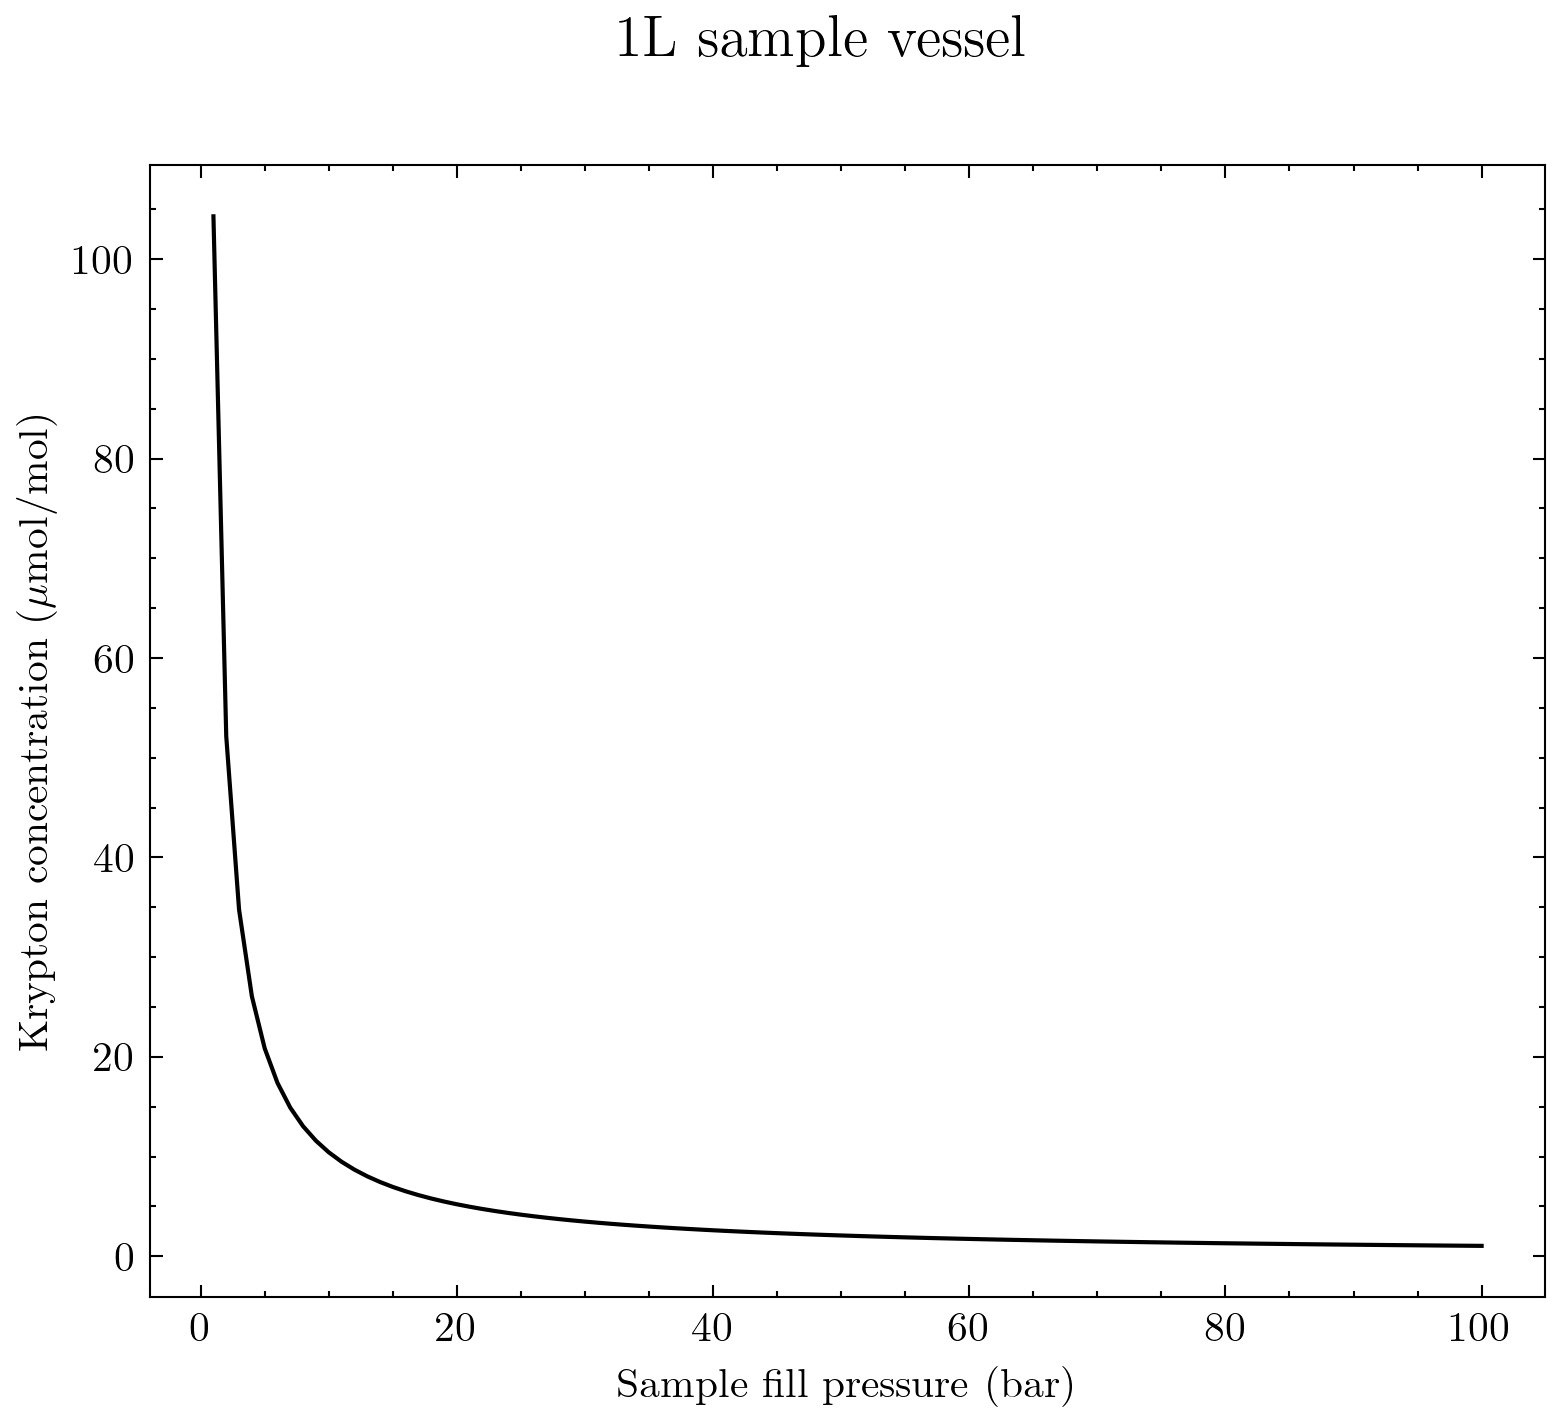
\includegraphics[width=0.5\linewidth, keepaspectratio]{/Users/marc/Thesis/Chapter5/1L.jpg}
    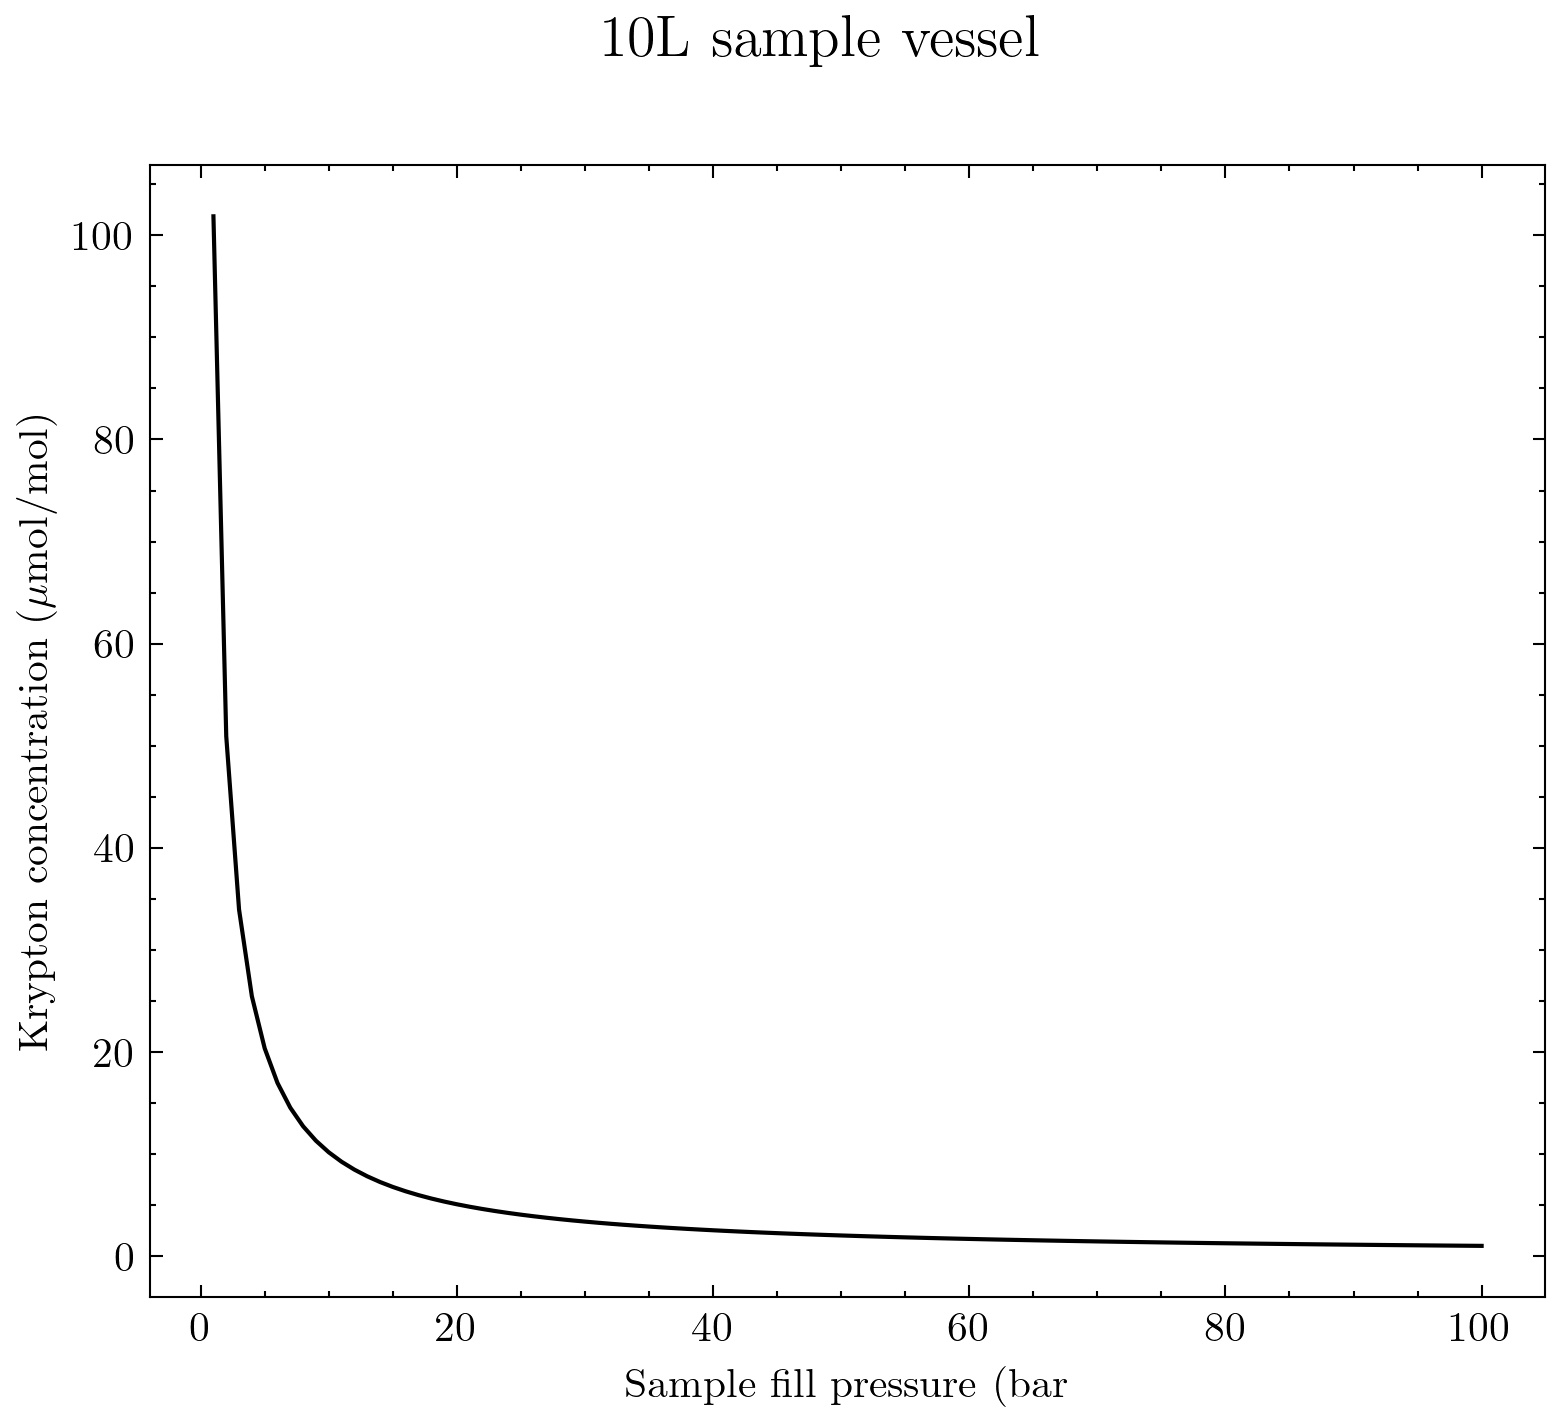
\includegraphics[width=0.5\linewidth, keepaspectratio]{/Users/marc/Thesis/Chapter5/10L.jpg}
    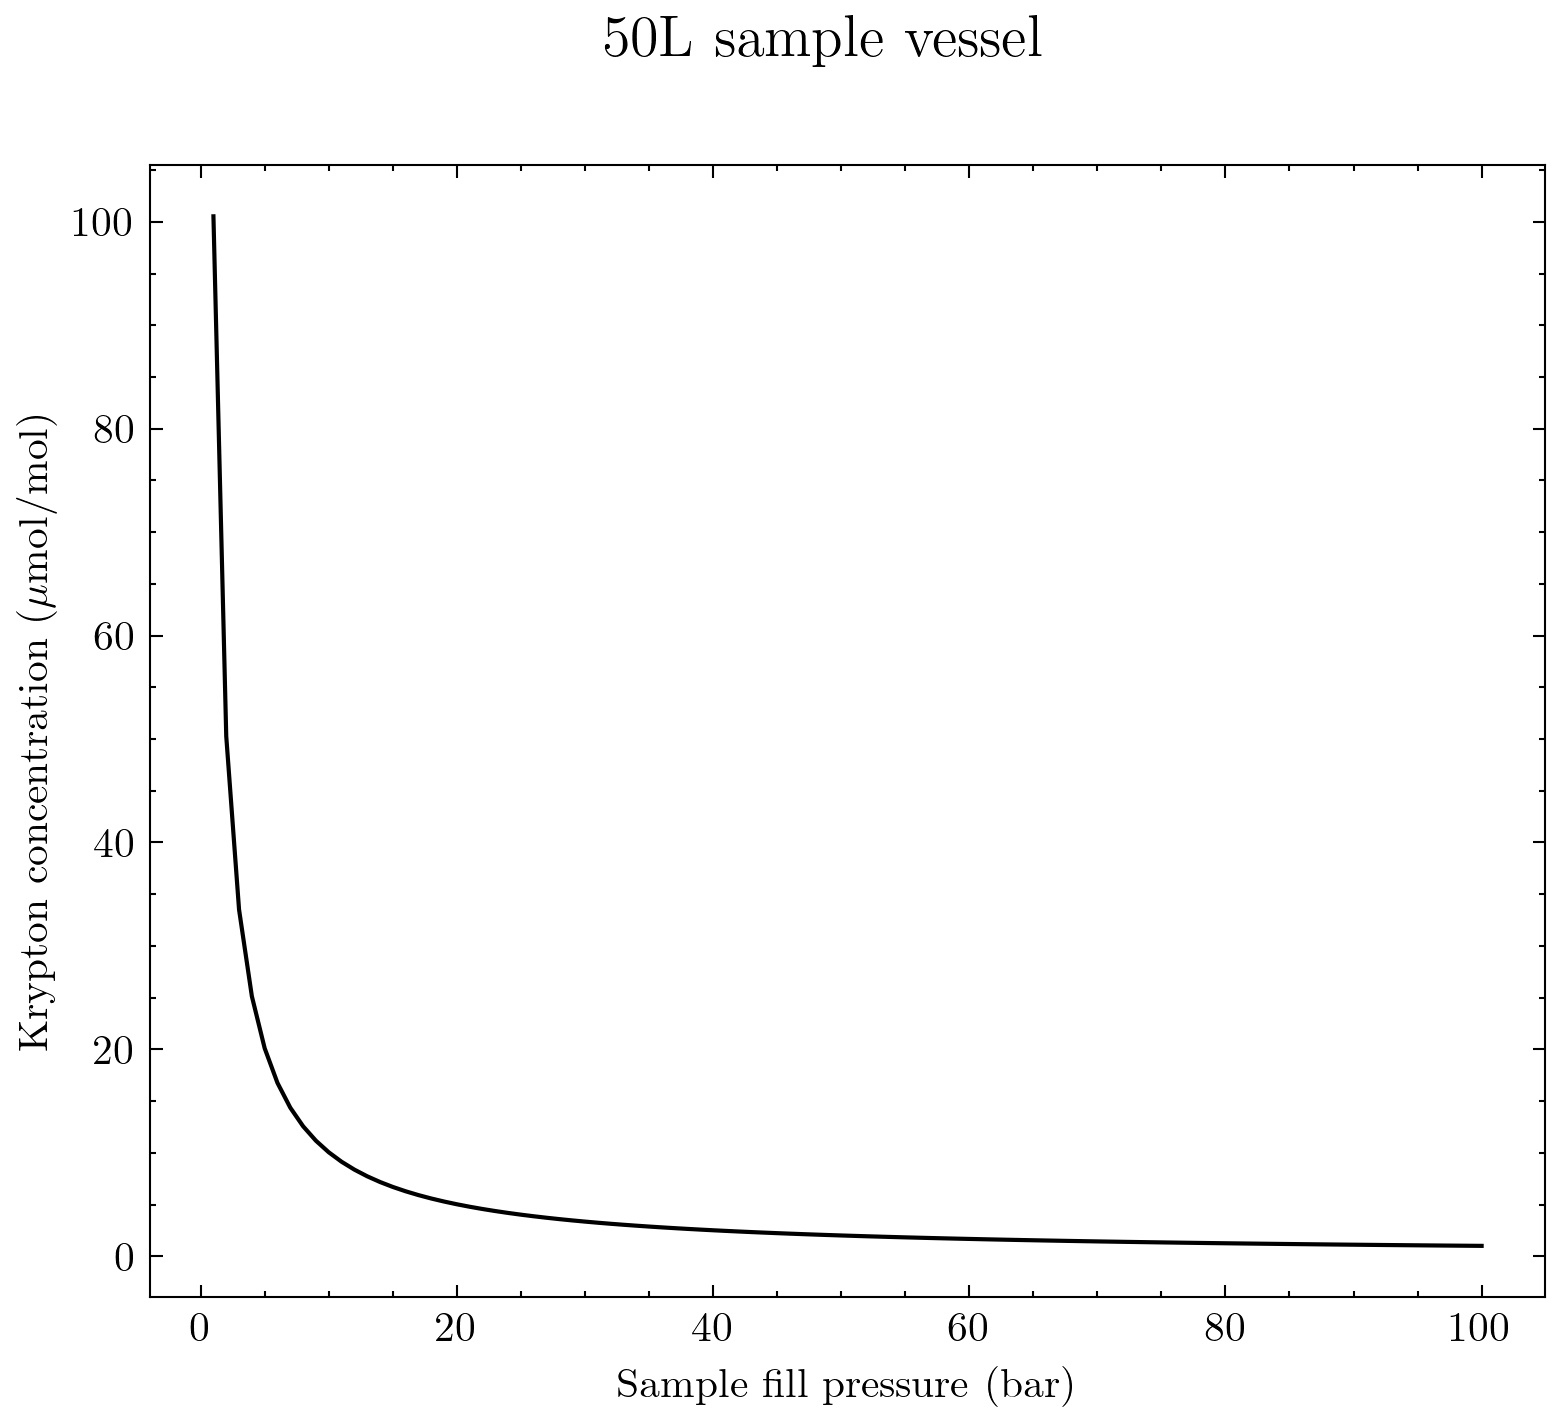
\includegraphics[width=0.5\linewidth, keepaspectratio]{/Users/marc/Thesis/Chapter5/50L.jpg}
    \caption{Predicted concentration of krypton within hydrogen samples in; 1L cylinder (30.8 mg Kr), 10L cylinder (300.79 mg Kr), 50L cylinder (1484 mg Kr)}
    \label{krsamples}
  \end{figure}

\section{Hydrogen Impurity enrichment device}
The aim of this section is to design an improved hydrogen impurity enrichment device which balances cost, accuracy and is operator-friendly. Automation will be taken into account in anticipation of the larger number of samples for analysis in the future and to improve the overall user experience. 
\subsection{Requirements}
Previous enrichment devices in literaure can be described as early prototypes.\cite{Ahmed2010} \cite{Murugan2014} In order to make the enrichment device commercially viable it must first be made more reliable. Greater control must be implemented over the pressures and temperatures within the device in order to ensure the membrane is not damaged inadvertently. Since the enrichment device operates by heating hydrogen to 300\textdegree C, adequate safety is of high concern. Previous enrichment devices in literature were lab scale, with the only safetry measures in place being those in the lab. Further safety and interlocks must be added to the enrichment device to ensure in the event of equipment failure the system can shut down safety. Finally all past devices involved the user manually recording important process values by hand, which is unintuitive, susceptible to errors, and does not allow easy monitoring system. An intuitive interface between the operator and the system will be added in order to automatically calculate output values such as the CEF, delivering this to the operator along with other important process parameters. 

\begin{itemize}
    \item Improve reliability by providing greater control over process parameters
    \item Improve safety by adding additional interlocks
    \item Improve user experience through in-situ process monitoring and data analysis
\end{itemize}

\subsection{System design}
The redesigned HIED is shown in figure \ref{hiedpid}. All tubing and pressure fittings were supplied by Swagelok \cite{swagelok} and the system was manufactured by Strata Technology London. \cite{stratatechnology}

The system is split into two units, the stationary unit and the transportable unit. The stationary unit is the bulk of the system, and contains piping to transport the gases to the enrichment device, connections for two gas cylinders for nitrogen (Q1) and the hydrogen sample to be tested (Q2), pressure relief valves (PSV001 \& PSV002), and connections to the vaccum system and gas vents. 

The transportable unit contains the enrichment vessel, heating and temperature control equipment, and the membrane. The enrichment vessel is a 300 cm\textsuperscript{3} sulfinert \cite{sulfinerttreatedsamplecylinder} treated vessel. The membrane is connected to one end of the vessel and operates in dead end mode. 

\subsubsection*{Safety}
It was decided that a nitrogen cylinder should be added to the system in order to ensure safety. Prior to evacuating the enrichment device the system should be purged 7 times with nitrogen  as this is adequate to reduce the concentration of gases remaining in the vessel, in particular the oxygen in air and any leftover hydrogen from previous tests, to a low enough level where it is not dangerous. \cite{BACQUART20205565} The enrichment device must be evacuated to a high vacuum before testing in order to ensure integrity of the results. Many commercially avaliable vacuum systems are not safe for use in explosive environments, therefore purging with nitrogen is a requirement before any procedures are to take place in the system. 

There are two pressure relief valves on the system. PSV001 is the safety interlock in the stationary unit and is set at 103 bar bar ensuring that in the event a higher pressure cylinder is connected to the system, there are sufficient safety measures in place. PSV002 is the pressure relief valve for the transportable unit, although is only in operation when it is connected to the stationary unit. and is set to 25 bar in order to prevent overpressurisation of the membrane. This pressure relief valve is critical when operating the enrichment device as the pressure initially in the enrichment vessel is at ambient conditions. As the enrichment vessel heats to the desired operating temperature, this pressure will increase, and since the enrichment vessel operates in dead end mode it is the only way out the system. This will cause the pressure within the enrichment vessel to potentially increase above the temperature rating of the membrane, resulting in failure. The pressure within the enrichment vessel is set using pressure controller PC001, effectivley creating two safety interlocks for the enrichment vessel. In the event of a pressure relief valve being triggered the gas will be automatically purged from the system through the vent.

\begin{landscape}
\begin{figure}
    \centering
    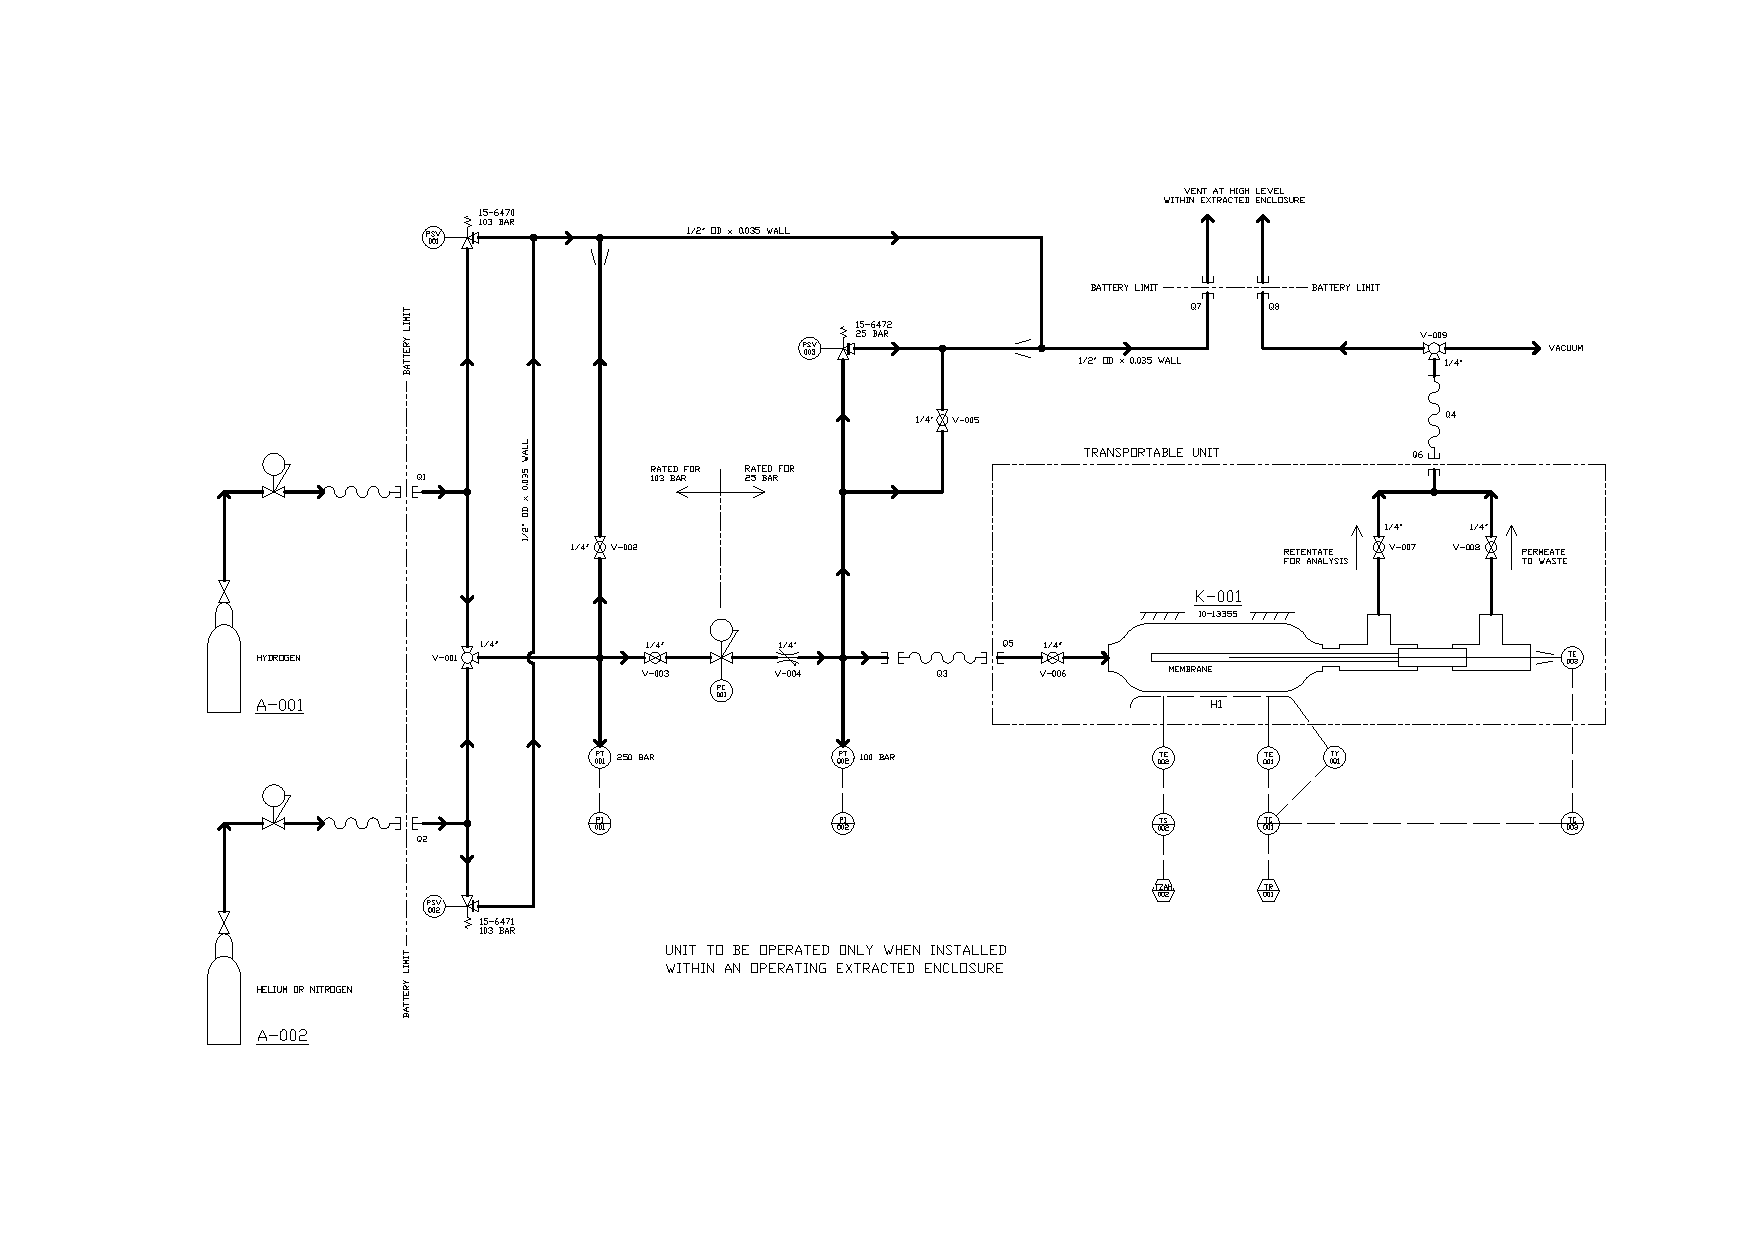
\includegraphics[height=0.5\pdfpageheight, keepaspectratio]{/Users/marc/Thesis/Chapter5/PID.pdf}
    \caption{P\&ID for the redesigned hydrogen impurity enrichment device}
    \label{hiedpid}
\end{figure}
\end{landscape}

\subsubsection*{User experience}
The main improvement to the user experience is through the segmentation of the system into the stationary unit and transportable unit which is shown in figure \ref{TU}. Bench space in a lab is often limited so often it is often not always possible to place the enrichment device next to the analyser that will be used following enrichment. Previous iterations of the enrichment device required either transporting the whole device, which is a difficult and potentially dangerous task, or disconnecting the swagelok fittings and transporting the vessel this way. While swagelok fittings can technically be disconected and reconnected, it is not reccomended since they are designed to be permenent pressure fittings, and the more times this operation is repeated, the faster components will have to be replaced. 

The transportable unit replaces these with VCR fittings, which are designed for disconnection and reconnection. The transportable unit also contains connections for the thermocouples connected to the temperature monitoring and control system, and the electrican connection to the system which are all designed for easy removal and reconnection. Finally the ergonomics of transporting the device have been improved through addition of a handle, allowing for eary transportation without unintentionally placing any strain on the pressure fittings. 
\begin{figure}
    \centering
    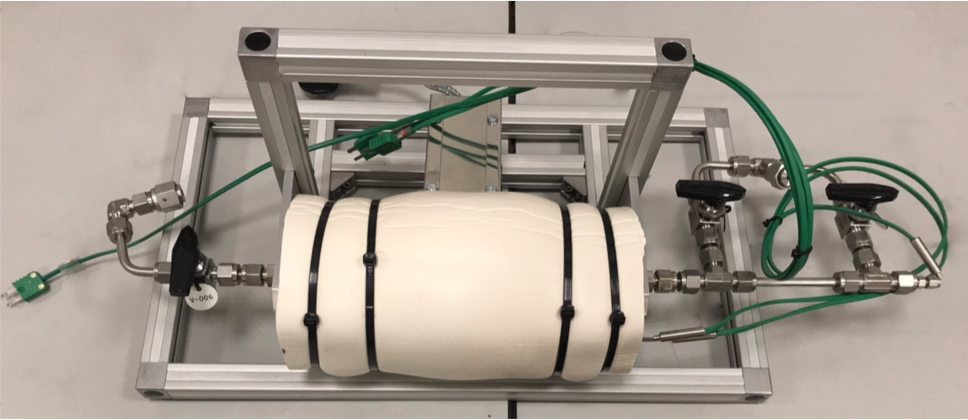
\includegraphics[width=\linewidth, keepaspectratio]{/Users/marc/Thesis/figures/TU.png}
    \caption{Disconnected transportable unit}
    \label{TU}
\end{figure}

\subsubsection*{Reliability}
The main improvement in reliability is a result of less instances of breaking and reconnecting fittings. As the system has been split into the stationary unit and transportable unit, the pressure fittings will gain an increased lifespan. Since the system is stationary it can benefit from being permenently connected to an evacuation rig and nitrogen supply. In the event of leakage multiple valves are implemented to allow the user to isolate different parts of the system in order to identify and replace the leaking component.

\subsection{Control/Measurement system}
There are two main factors to control for the enrichment device, the temperature and pressure. In past iterations of these systems control and measurement was done manually and hardwired into the system. By implementing adequate systems to measure and control these values operation of the system becomes easier, safer and more reliable 

The temperature of the enrichment vessel is changed using heating tape wrapped around the heating tape, and then covered in several layers of insulation. Pressure is controlled using a tamper proof temperature controller.  

\subsubsection*{Reliability}
The original system used an On/Off temperature controller, which simply measured the temperature using a thermocouple placed inside the membrane (TE003, figure \ref{hiedpid}), when the temperature rises above the setpoint the heater is switched off, when it drops below the heater is switched back on. The solution was unreliable, for example when the temperature setpoint was set at 300\textdegree C, the average value recorded was 302.7\textdegree C, with a standard deviation of 5\textdegree C. This is shown in figure \ref{TCcompare}. 

The system was upgraded with a PID temperature controller (OMRON), which continuously calculates an error value as the difference between a desired setpoint (SP) and a measured process variable (PV) and applies a correction based on proportional, integral, and derivative terms. This change in contro loop mechanism inproved the overall control of the system, bringing the average temperture recorded over 1 hour down to 302.7\textdegree C and the standard deviation down to 1.78\textdegree C.

\begin{figure}
    \centering
    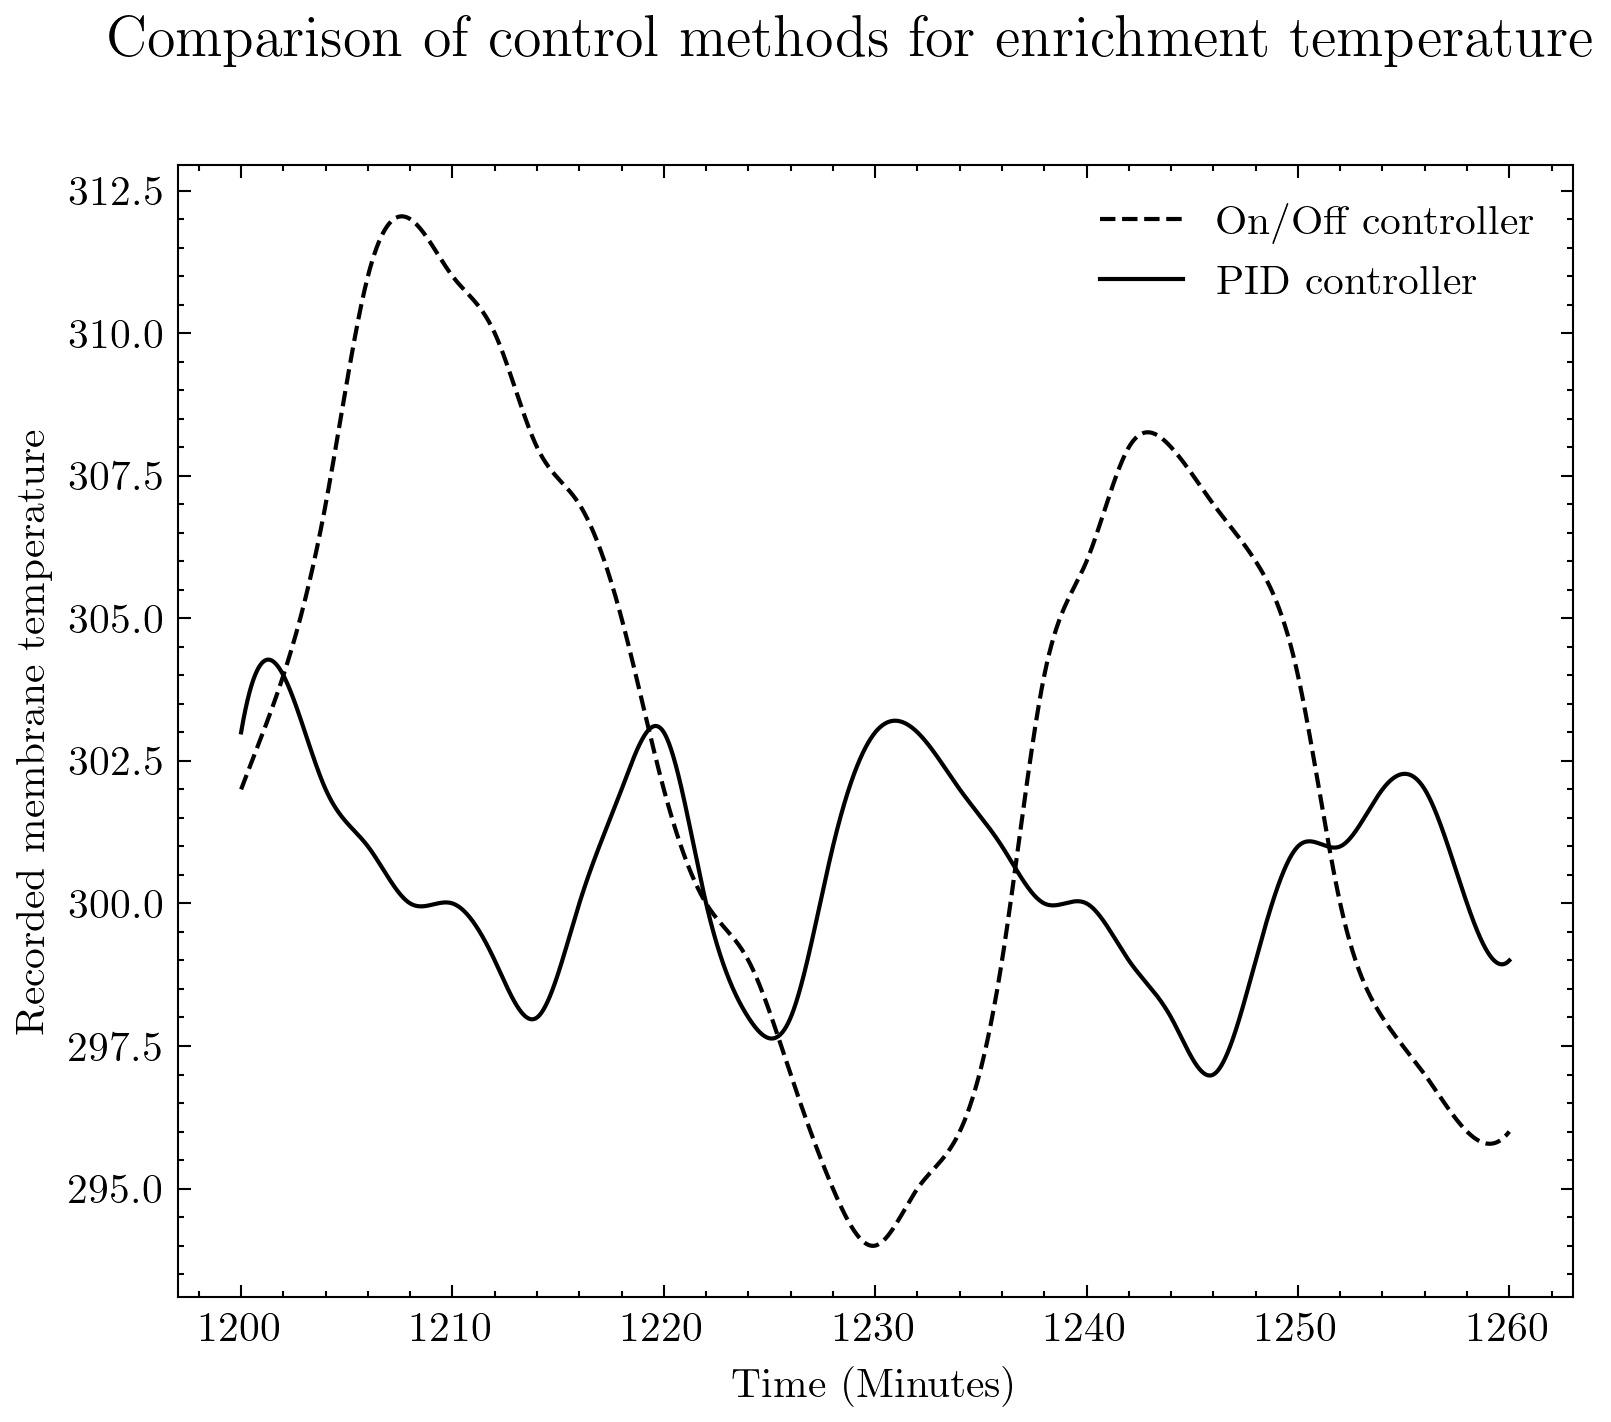
\includegraphics[width=\linewidth, keepaspectratio]{/Users/marc/Thesis/Chapter5/TC.jpg}
    \caption{Comparison of the On/Off temperature controller and PID temperature controller over a 1 hour period}
    \label{TCcompare}
\end{figure}

The pressure controller (PC001, figure \ref{hiedpid}) is considered reliable, as it can be set at a fixed pressure, which cannot be changed accidently by the user. The issue with reliability came from the measurement of pressure. Originally only one pressure sensor was used to measure the pressure inside the enrichment vessel (K-001), with the pressure of the sample cylinder used to calculate the enrichment factor only being measured once before and after the test. Two high resolution pressure sensors (Balluff) were added before and after the pressure controller so that both of these values could be monitored during the experiments. 

\subsubsection*{Safety}
The safety of the process was improved by adding a temperature shutoff to the enrichment vessel. There are three thermocouples (TE001, TE002 and TE003) on the enrichment vessel. TE003 is for controlling and monitoring the temperature of the membrane, while TE002 is for monitoring the temperature outside the vessell. TE003, which also measured the temperature outside the vessel, is connected to a temperature cut off, which is set 25\textdegree C above the setpoint temperature of the enrichment vessel. If the the recorded temperature outside of the enrichment vessel passes this threshold the heater will activate a trip, cutting off electricity until the device is checked by the operator. 

\subsubsection*{User experience}
The main improvement to user experience is the ability to easily control the temperature of the system. Previously the temperature controller was hardwired in, giving the user little control over the setpoint and temperature ramp of the device. With the new system these values can be controlled easily directly through the temperature controller, or using a microcontroller connected to the temperature controller, allowing for more options for the operator.

\subsection{Data processing}
Data collection and processing was done manually and no automation was involved. The main improvement in the new system involved the use of a microcontroller to automatically log process variables. These values were stored for later processing by the user. A data analysis script was also prepared in order to 

\section{Enrichment of hydrogen samples}

\subsection{Inert components}

\subsection{Sulphur containing compounds}

\subsection{HRS sample}

\section{Conclusion}
\bibliographystyle{unsrtnat}
\bibliography{library.bib}